% This must be in the first 5 lines to tell arXiv to use pdfLaTeX, which is strongly recommended.
\pdfoutput=1
% In particular, the hyperref package requires pdfLaTeX in order to break URLs across lines.

\documentclass[11pt]{article}

% Remove the "review" option to generate the final version.
\usepackage[review]{emnlp2021}

% Standard package includes
\usepackage{times}
\usepackage{latexsym}

% For proper rendering and hyphenation of words containing Latin characters (including in bib files)
\usepackage[T1]{fontenc}
% For Vietnamese characters
% \usepackage[T5]{fontenc}
% See https://www.latex-project.org/help/documentation/encguide.pdf for other character sets

% This assumes your files are encoded as UTF8
\usepackage[utf8]{inputenc}

% This is not strictly necessary, and may be commented out,
% but it will improve the layout of the manuscript,
% and will typically save some space.
\usepackage{microtype}
\usepackage{amsmath, amsfonts}
\usepackage{color}
\usepackage{graphicx}
\usepackage{tikz}
\usetikzlibrary{3d}
\usetikzlibrary{arrows.meta}
\usetikzlibrary{backgrounds}
\usetikzlibrary{bayesnet}
\usetikzlibrary{calc}
\usetikzlibrary{calligraphy}
\usetikzlibrary{fit}
\usetikzlibrary{positioning}
\usetikzlibrary{decorations.markings}
\usetikzlibrary{decorations.pathreplacing}
\usetikzlibrary{shapes}
\usetikzlibrary{shapes.geometric}
\usetikzlibrary{shapes.multipart}
\usetikzlibrary{tikzmark}
\usetikzlibrary{shapes}
\usetikzlibrary{shapes.geometric}
\usepackage{xspace}


\graphicspath{{images/}}
\DeclareGraphicsExtensions{.jpg,.png,.pdf}

\newcommand{\TODO}{\textcolor{red}{TODO}\xspace}
\newcommand\todo[1]{\textcolor{red}{#1}}
\newcommand{\ie}{i.e.,\xspace}

\usepackage{cleveref}
\usepackage{tabularx, booktabs}

% If the title and author information does not fit in the area allocated, uncomment the following
%
%\setlength\titlebox{<dim>}
%
% and set <dim> to something 5cm or larger.

\title{Learning Compositional Forms for Grounded Instructions}

% Author information can be set in various styles:
% For several authors from the same institution:
% \author{Author 1 \and ... \and Author n \\
%         Address line \\ ... \\ Address line}
% if the names do not fit well on one line use
%         Author 1 \\ {\bf Author 2} \\ ... \\ {\bf Author n} \\
% For authors from different institutions:
% \author{Author 1 \\ Address line \\  ... \\ Address line
%         \And  ... \And
%         Author n \\ Address line \\ ... \\ Address line}
% To start a seperate ``row'' of authors use \AND, as in
% \author{Author 1 \\ Address line \\  ... \\ Address line
%         \AND
%         Author 2 \\ Address line \\ ... \\ Address line \And
%         Author 3 \\ Address line \\ ... \\ Address line}

\author{First Author \\
  Affiliation / Address line 1 \\
  Affiliation / Address line 2 \\
  Affiliation / Address line 3 \\
  \texttt{email@domain} \\\And
  Second Author \\
  Affiliation / Address line 1 \\
  Affiliation / Address line 2 \\
  Affiliation / Address line 3 \\
  \texttt{email@domain} \\}

\begin{document}
\maketitle
\begin{abstract}
Young children who have mastered the compositionality of natural language are able to understand unfamiliar combinations of familiar words. 
%
In contrast, modern neural networks have been shown to struggle on tasks that require an ability to systematically generalize; so they fail when the train and test data contain the same set of words in the same semantic contexts, but certain classes of word combinations are held out from the training data.
%
These limitations are highlighted by a new challenge data-set \cite{ruis2020benchmark}, which tests for systematic generalization in a grounded setting by pairing natural language instructions  with executions in an environment. 
%
In this work, inspired by recent advances in language model pre-training \cite{devlin-etal-2019-bert} and multi-modal representations learning, we propose a new method for learning embeddings of the input natural language and environment together.
%
In our approach, the model learns generic grounded vision-and-text embeddings by pre-training on two tasks: (1) Grounded Masked Language Modeling (GMLM), in which the model uses  the visual input to infer masked words and (2) Language and Vision Inference (LVI), in which the model classifies whether a language instruction environment is relevant or not to a given environment.
%
These tasks require the resulting embeddings to capture information about the semantics of the instruction as they pertain to a particular visual environment.
%
Transformer-based sequence embeddings have been shown to capture complex dependencies between the words in a sentence, and we hypothesize that this strength will allow our approach to out-perform the RNN baseline presented in \cite{ruis2020benchmark}.
\end{abstract}

\section{Introduction}
Inspired by \cite{Lu2019ViLBERTPT} we devise a pre-training task that encourages our model to attend to the instruction and the environment jointly. 
%
At pre-training, the model receives the command and a representation of the initial environment. 
%
The model predicts whether a given command is relevant to the environment.
%
These embeddings will be used downstream by a planner (Section \ref{transformer-planner}) that will be trained to execute natural language structurions.
%
The hope is that these ``grounded'' embeddings will give our planner a head start in learning how the meaning of words can be composed.
%
One imagines that such a joint embedding will be helpful since knowing how to pick out the ``red'' items and the ``square''  items on a grid will be useful in picking out the ``red squares'', even if the phrase has never been seen before.

We will use the grounded-SCAN dataset \cite{ruis2020benchmark} which contains synthetic sentences paired with demonstrations in a grid world.
%
The sentences in the dataset are split so as to test the ability of a model to perform zero-shot generalization.
%
For example, the phrases ``red'', ``blue'', and ``blue square'' all appear in the training data, but the phrase ``red square'' appears only at test-time.

\section{Pre-training to improve grounding}
\begin{figure}
	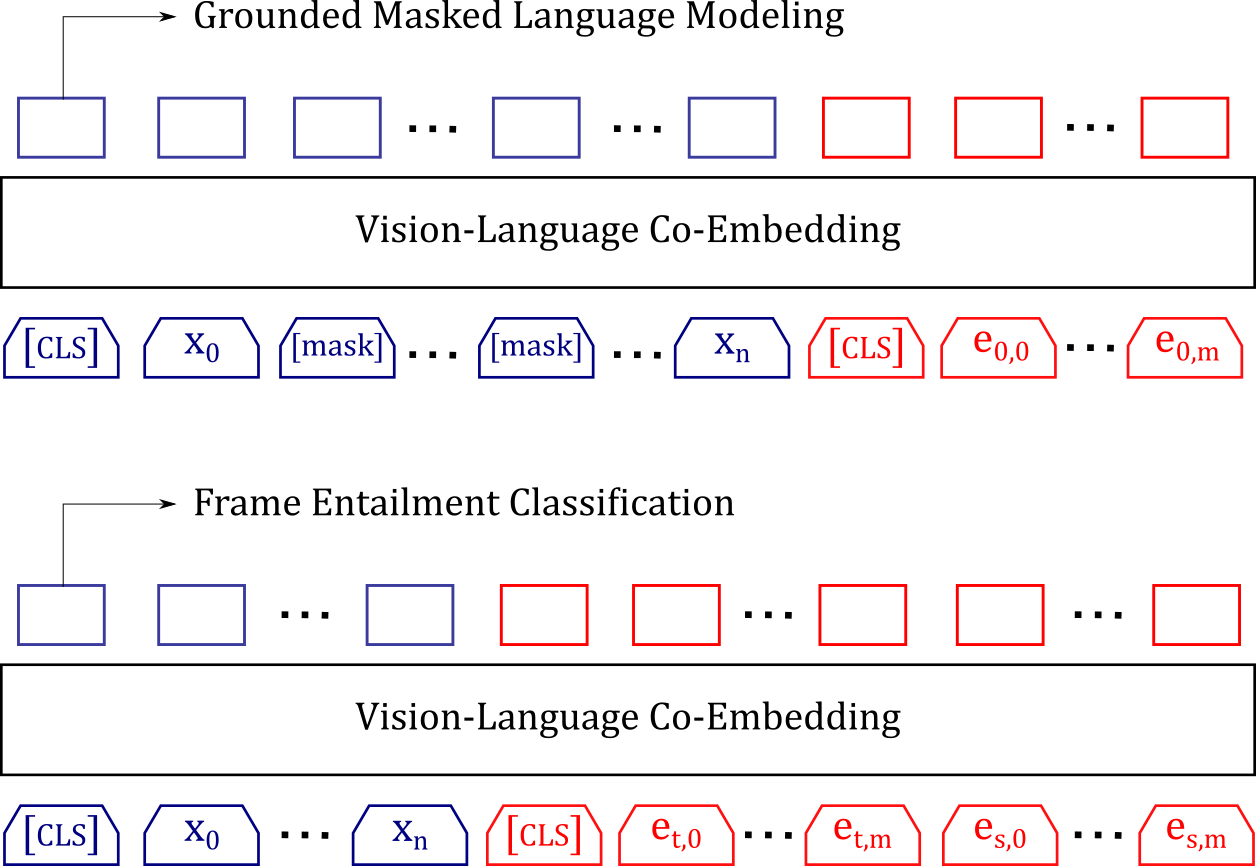
\includegraphics[width=3in]{pre_training_model.png}
	\caption{Two of our pre-training tasks. 
	%
	In Grounded Masked Language Modeling (top), the model receives the initial environment and the partially-masked command as input.
	%
	It must predict the masked portions of the input command.
	%
	In Frame Entailment Classification, the model receives the input command as well as visual representations from two frames of video data. 
	%
	It must classify the frames as being entailed by the command or not.
}
	\label{fig:pre_training}	
\end{figure}

\subsection*{Frame Entailment Prediction}
\todo{incomplete}
%
The model receives a natural language sentence and representations for the state of the world at two consecutive time-steps.
%
The model predicts whether the frames are entailed by the sentence.

\subsection{Multi-modal masked language modeling}
\todo{incomplete}
%
In the second masked language modeling task, we mask parts of the image as well as words of the sentence, and ask the model to fill in the missing words.

\section{Naturalistic data}
In order to test whether our model is capable of handling naturalistic language, we collected human-generated annotations via Amazon Mechanical Turk for each one of the test splits.
%
Note that the original sentences from \citet{ruis2020benchmark} are generated by a grammar.
%
Workers were shown the demonstration video and asked to write the sentence that might have produced the actions shown.
%
In order to preserve the compositional split, we also specified, per example, which properties of an object should not be mentioned.
%
Note that these sentences were used at test-time only.
%
Our experiment is to measure the performance of a model, trained on synthetic data, on naturalistic test data.
%
We hope to determine whether our model is truly capable of handling compositionality, as it is exhibited in natural human-generated language. 

\section{Multi-modal transformer baseline}
\label{transformer-planner}
\todo{incomplete}
We present our own simple planner to see if we can improve on the baseline given in \cite{ruis2020benchmark}.

\section{Related Work}
\subsection{Visual Language Navigation}
Our setting is very similar to the problem of Visual-Language-Navigation (VLN). 
%
In a VLN task, a robotic agent is given natural language directions to a specified goal location. 
%
The agent must navigate the environment until it reaches the goal.
%
With the advent of Transformers, many approaches have sought to build models for Visual-Language-Navigation \citep{magassouba2021crossmap, fang2019scene, Chen2020TopologicalPW}.
%
The problem that we focus on in this work is strictly more challenging than the VLN task. 
%
Not only must our agent learn to navigate, it must also learn to interact with the objects in the environment according to their attributes.

%
Our work is most related to the approach of \citet{Hao2020TowardsLA}, who present pre-training scheme to create embeddings for use in downstream Visual-Language-Navigation tasks.
%
But, their pre-training scheme relies on predicting an action for a given environment and instruction.
%
Our approach only relies on aligning commands to environments in which they are relevant, which is much less laborious to annotate.
%

\subsection{Transformers for Vision}
Our model takes both language and visual features as input, and thus builds on the work of \citep{LuViLBERT2019, tan-bansal-2019-lxmert, LiVisualBert2019}.

\subsection{Compositional Generalization}
The paper \citep{ruis2020benchmark} that introduced gSCAN also presented a simple baseline model.
%
Since then, numerous improvements on that model have been made \citep{gao-etal-2020-systematic, heinze-think-2020, kuo2020compositional}.
%
However, none of these improvements make use of recent advances in pre-trained language models. 

\section{Data}
Our model is trained on the grounded SCAN benchmark \citep{ruis2020benchmark}, a dataset of synthetic sentences in English paired with demonstrations in a grid world that systematically tests generalizations.
%
We collect a new dataset, grounded SCAN Human (\TODO name), which augments the demonstrations with human generated sentences.
%

\subsection*{A. Random}
The random test split simply verifies that in the absence of controls, the model is able to learn all the conditions from the other splits. 

\subsection*{B,C. Novel attribute composition}
In (B), in the train set, a yellow square can be the target object, but is never referred to by color. 
%
At test time, the model must ground the reference ``yellow square.''

In (C), in the train set, the red square is never the target object.
%
However, the agent may still encounter red or square objects.

\subsection*{D. Novel direction}
In this split, the target object is never to the south-west of the agent's initial position.

\subsection*{E. Novel contextual reference}
During training, the model sees, and receives references to, a circle of size 2, but the model is never the smallest circle and is never referred to as the "small circle".
%
At test time, the model must learn to identify the circle of size 2 as the ``small circle."

\subsection*{F. Novel composition of actions and arguments}
At train time, the model never has to `push' a heavy square.
%
However, it learns to `pull' a heavy square, and how to `push' a heavy cylinder.
%
At test time, it is asked to `push' a heavy square.

\subsection*{G,H. Novel Adverbs}
In (H), the train split contains the verb `pull' and the adverb `while spinning', but never together. 
%
The model must execute `pull while spinning' correctly at test time. 

In (G), the train split contains a few examples of the adverb `cautiously', and in the test set, the model must demonstrate an ability to understand the adverb in all contexts.

\section{Model Architecture}
The training data $D=\{(\mathbf{x}_i, E_i) \}_{i=1}^{i=|D|}$ consists of natural language commands $\mathbf{x}$ paired with an execution $E$. 
%
Each execution $E$ is a tuple of a sequence, $\mathbf{a}$, with $T$ actions and a sequence, $\mathbf{e}$, with $T+1$ environments, where action $\mathbf{a}_t$ results in state  $\mathbf{e}_{t+1}$. 
%
Each environment is represented by $m$ image patches: $\mathbf{e}_{t} = [e_{t,0}\cdots e_{t,m}]$.
%

\Cref{fig:training_model} shows our model as it makes a forward pass during training.
%
Consider an input command $\mathbf{x}_{i}$ of length $n$.
%
At each time-step $t$, the model receives patches $\mathbf{e}_t$ which represent the environment as it appears in that moment. 
%
The command and patches are embedded using a text and vision embedding layer, respectively. 
%
The embeddings are passed to stacked co-transformer and transformer layers, which alternately attend to one and both input modalities.
%
Each co-Transformer also attends to the top-most hidden state representations of the previous time-step.
%
(\todo{TODO: does each co-Transformer in the stack attend to the same hidden states, or only the bottom layer?})
%
The topmost of the stacked transformers outputs a representation of the text as a sequence of $n$ hidden states, $[h_{[CLS]}^l,\cdots,h_{n}^l]$, and a representation of the image patches as $m$ hidden states $[h^e_{[CLS]}, \cdots, h^{e}_{m}]$.
%
A context vector $c_t$ is formed by concatenating $h_{[CLS]}^l$ and $h_{[CLS]}^e$.
%
The context vector passes through a linear projection layer and Softmax, producing a distribution over actions, from which $a_t$ is selected.
%
Decoding precedes auto-regressively.

\begin{figure}
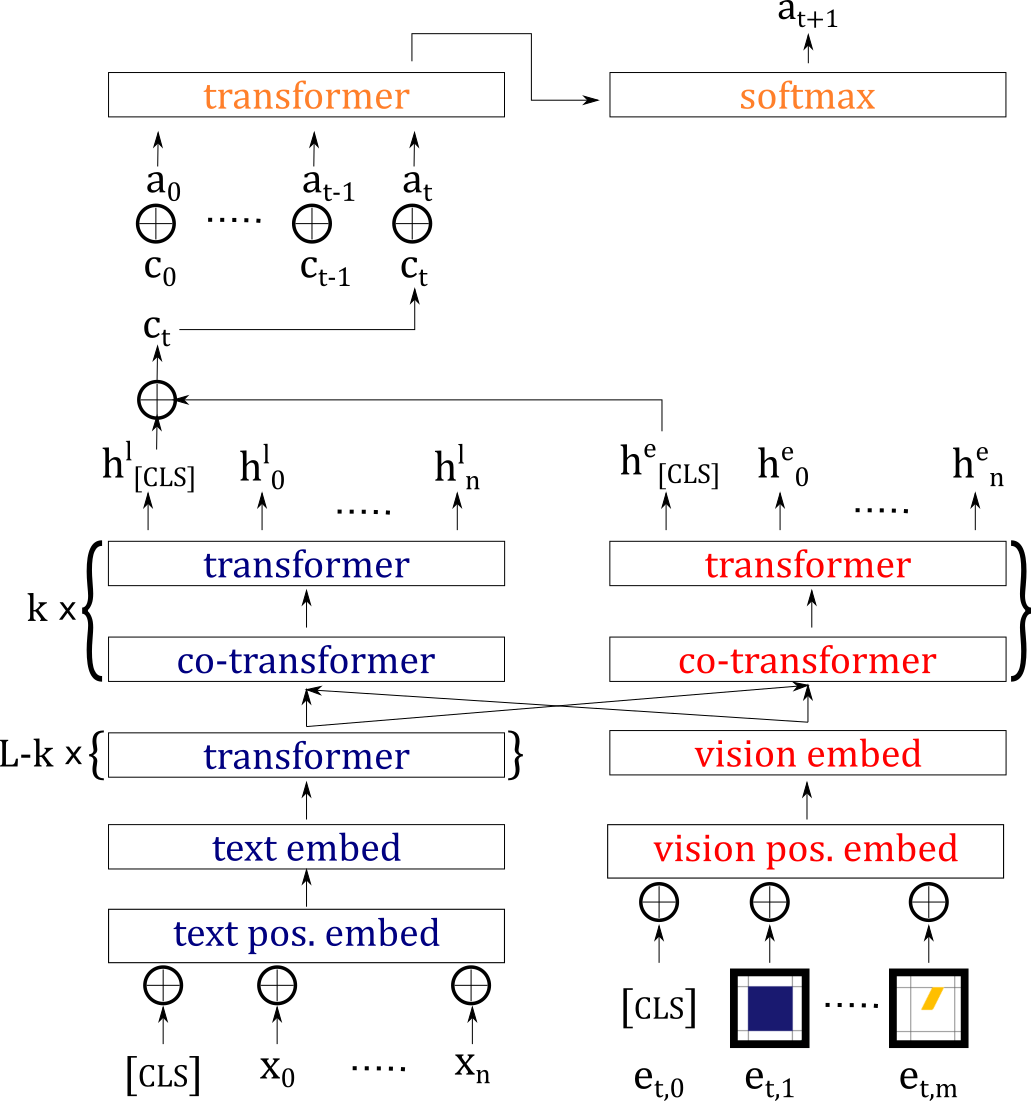
\includegraphics[width=3in]{training_model.png}
\caption{Predicting an action at time $t$. Our model consists of a text encoder (blue), a vision encoder (red), and an action decoder (orange). }
\label{fig:training_model}	
\end{figure}

\subsection{Cross-Attention}
A Transformer layer takes an input sequence of vectors $\mathbf{Q}$, called the query vectors. 
%
For each $q\in \mathbf{Q}$, a context vector is created from a weighted sum of vectors $\mathbf{V}$, called the value vectors.
%
The weights in this sum are generated by taking the dot product between $\mathbf{Q}$ and $\mathbf{K}$, where $\mathbf{K}$ is the set of key vectors that represent $\mathbf{V}$.

In cross-attention, the language co-Transformer takes $\mathbf{Q}_{l}$, $\mathbf{V}_{v}$, $\mathbf{K}_{v}$ as input, where $\mathbf{Q}_l$ are the hidden states of the text Transformer, and $\mathbf{K}_{v}$ and $\mathbf{V}_{v}$ are the hidden states of the vision Transformer.

\section{RNN baseline}
We compare our model with an RNN decoder to show the effectiveness (1) of our pre-training scheme and (2) of our Transformer-based action decoder.
%

We run two experiments.
%
In the first experiment, we first pre-trained our text and vision encoder using grounded masked language modeling. 
%
In the second experiment, we instead use randomly initialized weights for our text and vision encoder.

%
At inference time, the model receives the text and vision encoder create text embeddings, $[h_{[CLS]}^{l},...,h_{n}^{l}]$, for the input command and vision embeddings, $[h_{[CLS]}^{v},...,h_{m}^{v}]$ for the patches for the initial grid.
%
At each time-step $t$, the RNN receives these embeddings, as well as the image features of the environment at that time-step $e_t$.
%
A context vector $c_t$ is created by applying attention to the input embeddings, using the prior hidden state $h_{t-1}$ as the query vector:
\begin{align*}
c_{t,v} &= \text{Attn}_v(h_{t-1}, [h_{[CLS]}^{v},...,h_{m}^{v}])\\
c_{t,l} &= \text{Attn}_l(h_{t-1}, [h_{[CLS]}^{l},...,h_{n}^{l}])\\
c_t &= c_{t,v} + c_{t,l}
\end{align*}
Given this context vector and the previous hidden state $h_{t}$ as input, the RNN produces a new hidden state $h_{t+1}$:
$$
h_{t+1} = RNN(h_t, c_t)
$$
The hidden state at time $t$, $h_t$ is fed through a fully-connected layer, and a softmax is used to produce a distribution over actions, from which the action $a_t$ is sampled:
$$
p(a_{t+1} \mid a_{0:t}, e_{0:t}, x) = \text{Softmax}(FC(h_{t+1}))
$$
%

\Cref{tab:gscan_results} shows the performance of our baseline.

\begin{table*}
\begin{center}
\begin{tabularx}{\textwidth}{ l|ccccccccc }
\toprule
\multicolumn{1}{c}{} 
& \multicolumn{4}{c}{Transformer}  
& \multicolumn{4}{c}{RNN}  
& \\
\cmidrule{3-4}
\cmidrule{7-8}
\multicolumn{1}{c}{} 
& \multicolumn{2}{c}{w/ pre-training}  
& \multicolumn{2}{c}{random}
& \multicolumn{2}{c}{w/ pre-training}  
& \multicolumn{2}{c}{random}
& \multicolumn{1}{c}{\cite{ruis2020benchmark}}\\
& test  & val  & test &  val & test &  val & test & val & test  \\
\midrule
A: Random & --  & --  & -- &  -- & -- &  -- & -- &  -- & 97.69 $\pm$ 0.22\\
B: Yellow Squares & --  & --  & -- &  -- & -- &  -- & -- &  -- &  54.96 $\pm$ 39.39\\
C: Red Squares & --  & --  & -- &  -- & -- &  -- & -- &  -- & 23.51 $\pm$ 21.82\\
D: Novel Direction & --  & --  & -- & -- & -- &  -- & -- &  -- & 0.00 $\pm$ 0.00 \\
E: Relativity & --  & --  & -- & -- & -- &  -- & -- &  -- & 35.02 $\pm$ 2.35 \\
F: Class Inference & --  & --  & -- &  -- &-- &  -- & -- &  -- &  92.52 $\pm$ 6.75 \\
H: Adverb to Verb & --  & --  & -- &  -- &-- &  -- & -- &  -- &  92.52 $\pm$ 6.75 \\
\bottomrule
\end{tabularx}
\end{center}
\caption{The performance of our model and our RNN baseline on the gSCAN splits. We show the difference that results from using our pre-training scheme.}
\label{tab:gscan_results}
\end{table*}

\begin{table*}
	\begin{center}
		\begin{tabularx}{\textwidth}{ l|ccccccccc }
			\toprule
			\multicolumn{1}{c}{} 
			& \multicolumn{4}{c}{Transformer}  
			& \multicolumn{4}{c}{RNN}  
			& \\
			\cmidrule{3-4}
			\cmidrule{7-8}
			\multicolumn{1}{c}{} 
			& \multicolumn{2}{c}{w/ pre-training}  
			& \multicolumn{2}{c}{random}
			& \multicolumn{2}{c}{w/ pre-training}  
			& \multicolumn{2}{c}{random}
			& \multicolumn{1}{c}{\cite{ruis2020benchmark}}\\
			& test  & val  & test &  val & test &  val & test & val & test  \\
			\midrule
			A: Random & --  & --  & -- &  -- & -- &  -- & -- &  -- & 97.69 $\pm$ 0.22\\
			B: Yellow Squares & --  & --  & -- &  -- & -- &  -- & -- &  -- &  54.96 $\pm$ 39.39\\
			C: Red Squares & --  & --  & -- &  -- & -- &  -- & -- &  -- & 23.51 $\pm$ 21.82\\
			D: Novel Direction & --  & --  & -- & -- & -- &  -- & -- &  -- & 0.00 $\pm$ 0.00 \\
			E: Relativity & --  & --  & -- & -- & -- &  -- & -- &  -- & 35.02 $\pm$ 2.35 \\
			F: Class Inference & --  & --  & -- &  -- &-- &  -- & -- &  -- &  92.52 $\pm$ 6.75 \\
			H: Adverb to Verb & --  & --  & -- &  -- &-- &  -- & -- &  -- &  92.52 $\pm$ 6.75 \\
			\bottomrule
		\end{tabularx}
	\end{center}
	\caption{The performance of our model and baseline RNN decoder on human annotated data.}
	\label{tab:human_results}
\end{table*}

\begin{table*}
	\begin{center}
		\begin{tabularx}{\textwidth}{ l|cccccccc}
			\toprule
			\multicolumn{1}{c}{} 
			& \multicolumn{2}{c|}{BERT}  
			& \multicolumn{2}{c|}{-vis. pre-train}  
			& \multicolumn{2}{c|}{-mult. frame pre-train}  
			& \multicolumn{2}{c|}{-vis. train} \\
			& test  & val  & test &  val & test &  val & test & val \\
			\midrule
			A: Random & --  & --  & -- &  -- & -- &  -- & -- &  -- \\
			B: Yellow Squares & --  & --  & -- &  -- & -- &  -- & -- &  -- \\
			C: Red Squares & --  & --  & -- &  -- & -- &  -- & -- &  -- \\
			D: Novel Direction & --  & --  & -- & -- & -- &  -- & -- &  --  \\
			E: Relativity & --  & --  & -- & -- & -- &  -- & -- &  --  \\
			F: Class Inference & --  & --  & -- &  -- &-- &  -- & -- &  --  \\
			H: Adverb to Verb & --  & --  & -- &  -- &-- &  -- & -- &  -- \\
			\bottomrule
		\end{tabularx}
	\end{center}
	\caption{Various ablations of our model. In the first column, we use the pre-trained BERT weights only for our embedding. For the second, we do not feed any visual input to the model during pre-training. For the third, we only give the initial environment state to the model during pre-training. For the fourth, we do not give the model visual input during training.}
	\label{tab:ablations}
\end{table*}


\subsection{Results}

\subsection{Discussion}



% Entries for the entire Anthology, followed by custom entries
\bibliography{anthology,custom}
\bibliographystyle{acl_natbib}

\appendix

\section{Example Appendix}
\label{sec:appendix}

This is an appendix.

\end{document}
